% !Mode:: "TeX:UTF-8"
\chapter{SLAM:现在与未来}
\begin{mdframed}  
	\textbf{主要目标}
	\begin{enumerate}[labelindent=0em,leftmargin=1.5em]
		\item 了解经典的SLAM实现方案。
		\item 通过实验,比较各种SLAM方案的异同。
		\item 探讨SLAM的未来发展方向。
	\end{enumerate}
\end{mdframed}

前面介绍了一个SLAM系统中的各个模块的工作原理,这是研究者们多年工作的结晶。目前,除了这些理论框架之外,我们也积累了许多优秀的开源SLAM方案。不过,由于它们大部分的实现都比较复杂,不适合作为初学者的上手材料,所以我们放到了本书的最后加以介绍。相信读者通过阅读之前的内容,应该能明白其基本原理。

\newpage 
\section{当前的开源方案}
本讲是全书的总结,我们将带着读者去看看现有的SLAM方案能做到怎样的程度。特别地,我们重点关注那些提供开源实现的方案。在SLAM研究领域,能见到开源方案是很不容易的。往往论文中介绍理论只占20\%的内容,其他80\%都写在代码中,是论文里没有提到的。正是这些研究者们的无私奉献,推动了整个SLAM行业的快速前进,使后续研究者有了更高的起点。在我们开始做SLAM之前,应该对相似的方案有深入的了解,然后再进行自己的研究,这样才会更有意义。

本讲的前半部分将带领读者参观一下当前的视觉SLAM方案,评述其历史地位和优缺点。\autoref{table:opensource-slam}~列举了一些常见的开源SLAM方案,读者可以选择感兴趣的方案进行研究和实验。限于篇幅,我们只选了一部分有代表性的方案,这肯定是不全面的。在后半部分,我们将探讨未来可能的一些发展方向,并给出当前的一些研究成果。

{
\small
\begin{table}[!h]
\caption{常用开源SLAM方案}
\label{table:opensource-slam}
\begin{tabu}{@{}c|c|X@{}}
\toprule
	方案名称 & 传感器形式 & 地址 \\
\midrule
	MonoSLAM &  单目 & \url{https://github.com/hanmekim/SceneLib2}  \\ 
	PTAM & 单目 & \url{http://www.robots.ox.ac.uk/~gk/PTAM/} \\ 
	ORB-SLAM & 单目为主 & \url{http://webdiis.unizar.es/~raulmur/orbslam/} \\ 
	LSD-SLAM & 单目为主 & \url{http://vision.in.tum.de/research/vslam/lsdslam} \smallskip \\
	SVO & 单目 & \url{https://github.com/uzh-rpg/rpg_svo} \\ 
	DTAM & RGB-D & \url{https://github.com/anuranbaka/OpenDTAM} \\ 
	DVO & RGB-D & \url{https://github.com/tum-vision/dvo_slam} \\ 
	DSO & 单目 & \url{https://github.com/JakobEngel/dso} \\
    VINS系列 & 单目+IMU为主 & \url{https://github.com/HKUST-Aerial-Robotics/VINS-Mono} \\
	RTAB-MAP & 双目/RGB-D & \url{https://github.com/introlab/rtabmap} \\ 
	RGBD-SLAM-V2 & RGB-D & \url{https://github.com/felixendres/rgbdslam_v2} \\ 
	Elastic Fusion & RGB-D & \url{https://github.com/mp3guy/ElasticFusion} \\ 
	Hector SLAM & 激光 & \url{http://wiki.ros.org/hector_slam} \\ 
	GMapping & 激光 & \url{http://wiki.ros.org/gmapping} \\ 
	OKVIS & 多目+IMU & \url{https://github.com/ethz-asl/okvis} \\ 
	ROVIO & 单目+IMU & \url{https://github.com/ethz-asl/rovio} \\ 
\bottomrule
\end{tabu}
\end{table}
}

\smallskip
\subsection{MonoSLAM}
说到视觉SLAM,很多研究者第一个想到的是A. J. Davison的单目SLAM工作\textsuperscript{\cite{Davison2007,Davison2003}}。Davison教授是视觉SLAM研究领域的先驱,他在2007年提出的MonoSLAM是第一个实时的单目视觉SLAM系统\textsuperscript{\cite{Davison2007}},被认为是许多工作的发源地\footnote{这是他博士期间工作的延续。他现在也在致力于将SLAM小型化、低功率化。}。MonoSLAM以扩展卡尔曼滤波为后端,追踪前端非常稀疏的特征点。由于EKF在早期SLAM中占据着明显主导地位,所以MonoSLAM亦是建立在EKF的基础之上,以相机的当前状态和所有路标点为状态量,更新其均值和协方差。

\autoref{fig:mono-slam}~所示是MonoSLAM在运行时的情形。可以看到,单目相机在一幅图像当中追踪了非常稀疏的特征点(且用到了主动追踪技术)。在EKF中,每个特征点的位置服从高斯分布,所以我们能够以一个椭球的形式表达它的均值和不确定性。在该图的右半部分,我们可以找到一些在空间中分布着的小球。它们在某个方向上显得越长,说明在该方向的位置就越不确定。我们可以想象,如果一个特征点收敛,我们应该能看到它从一个很长的椭球(相机$Z$方向上非常不确定)最后变成一个小点的样子。

\begin{figure}[!htp]
	\centering
	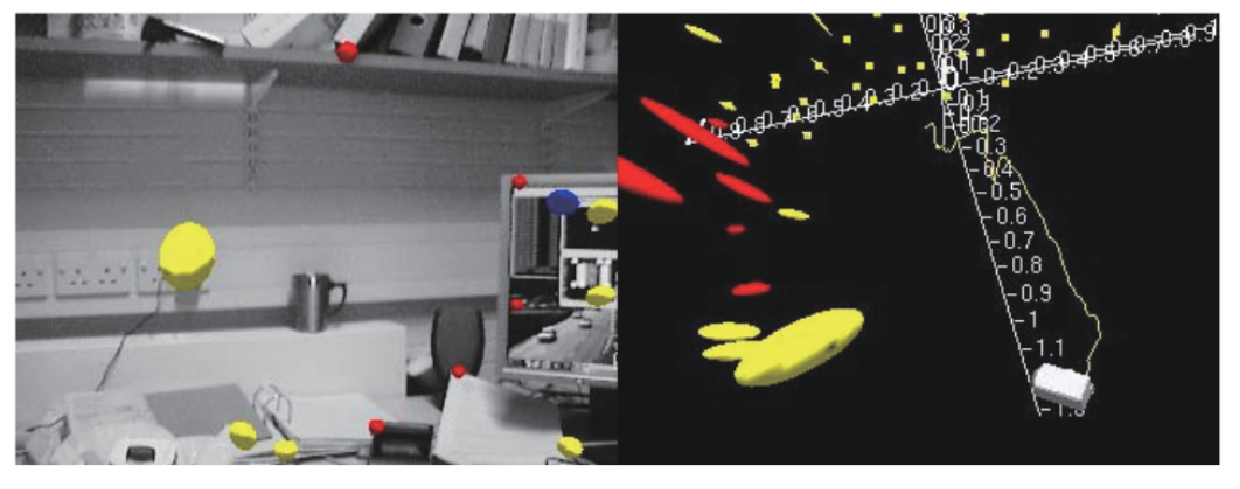
\includegraphics[width=1.0\textwidth]{past-and-future/mono-slam.pdf}
	\caption{MonoSLAM的运行时截图。左侧:追踪特征点在图像中的表示; 右侧:特征点在三维空间中的表示。}
	\label{fig:mono-slam}
\end{figure}

这种做法在今天看来固然存在许多弊端,但在当时已经是里程碑式的工作了,因为在此之前的视觉SLAM系统基本不能在线运行,只能靠机器人携带相机采集数据,再离线地进行定位与建图。计算机性能的进步,以及用稀疏的方式处理图像,加在一起才使得一个SLAM系统能够在线地运行。从现代的角度来看,MonoSLAM存在诸如应用场景很窄,路标数量有限,稀疏特征点非常容易丢失的情况,对它的开发也已经停止,取而代之的是更先进的理论和编程工具。不过这并不妨碍我们对前人工作的理解和尊敬。

\subsection{PTAM}

2007年,Klein等人提出了PTAM(Parallel Tracking and Mapping)\textsuperscript{\cite{Klein2007}},这也是视觉SLAM发展过程中的重要事件。PTAM的重要意义在于以下两点:
\begin{enumerate}
	\item PTAM提出并实现了跟踪与建图过程的并行化。我们现在已然清楚,跟踪部分需要实时响应图像数据,而对地图的优化则没必要实时地计算。后端优化可以在后台慢慢进行,然后在必要的时候进行线程同步即可。这是视觉SLAM中首次区分出前后端的概念,引领了后来许多视觉SLAM系统的设计(我们现在看到的SLAM多半都分前后端)。
	\item PTAM是第一个使用非线性优化,而不是使用传统的滤波器作为后端的方案。它引入了关键帧机制:我们不必精细地处理每一幅图像,而是把几个关键图像串起来,然后优化其轨迹和地图。早期的SLAM大多数使用EKF滤波器或其变种,以及粒子滤波器等;在PTAM之后,视觉SLAM研究逐渐转向了以非线性优化为主导的后端。由于之前人们未认识到后端优化的稀疏性,所以觉得优化后端无法实时处理那样大规模的数据,而PTAM则是一个显著的反例。

	\hspace{2em}PTAM同时是一个增强现实软件,演示了酷炫的AR效果(如\autoref{fig:ptam}所示)。根据PTAM估计的相机位姿,我们可以在一个虚拟的平面上放置虚拟物体,看起来就像在真实的场景中一样。
\end{enumerate}

\begin{figure}[!ht]
	\centering
	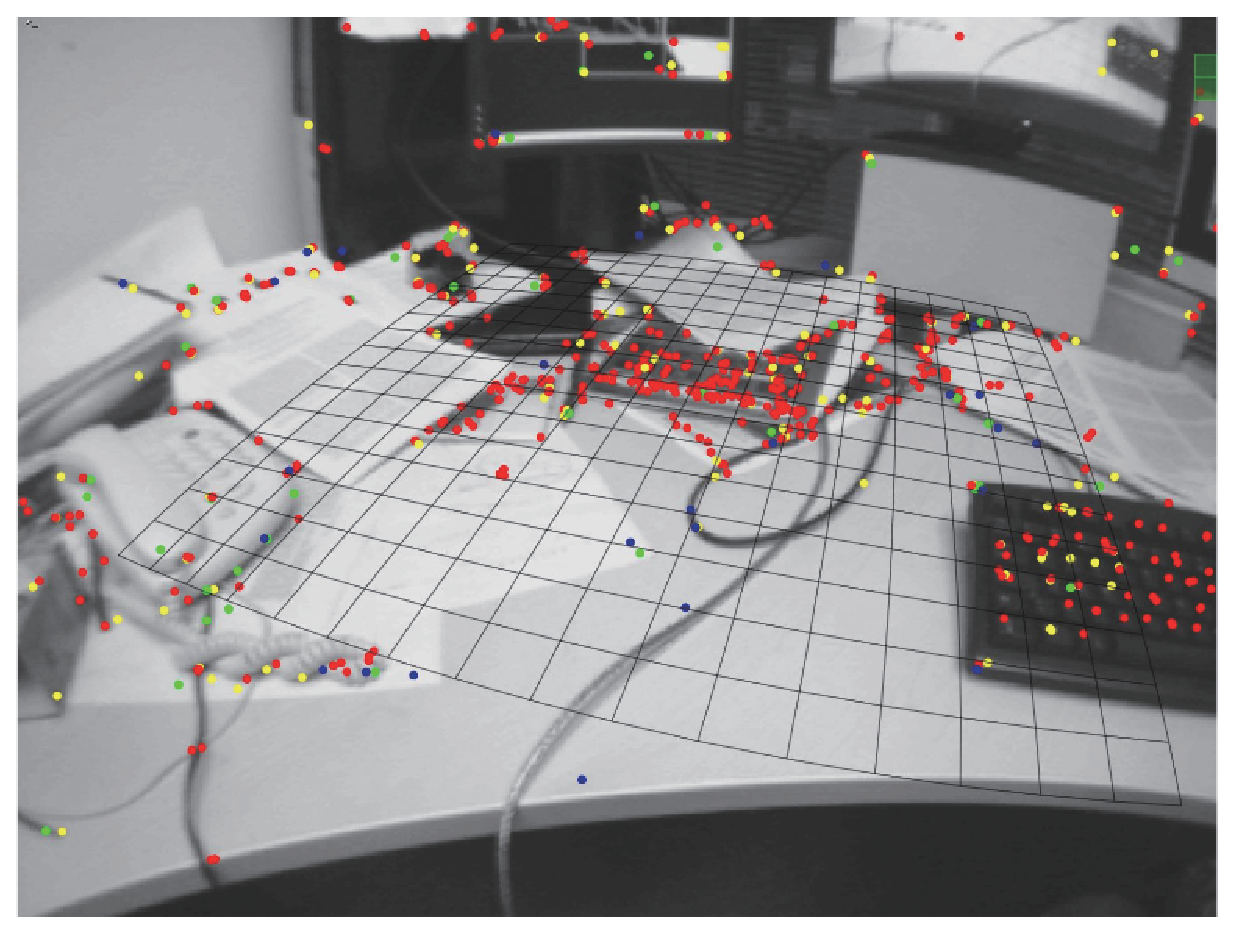
\includegraphics[width=1.0\textwidth]{past-and-future/ptam}
	\caption{PTAM的演示截图。它既可以提供实时的定位和建图,也可以在虚拟平面上叠加虚拟物体。}
	\label{fig:ptam}
\end{figure}

\clearpage
不过,从现代的眼光看来,PTAM也算是早期的结合AR的SLAM工作之一。与许多早期工作相似,存在着明显的缺陷:场景小,跟踪容易丢失,等等。这些又在后续的方案中得以修正。

\subsection{ORB-SLAM}

介绍了历史上的几种方案之后,我们来看现代的一些SLAM系统。ORB-SLAM是PTAM的继承者中非常有名的一位\textsuperscript{\cite{Mur-Artal2015}}(见\autoref{fig:orb-slam})。它提出于2015年,是现代SLAM系统中做得非常完善、非常易用的系统之一(如果不是最完善易用的话)。ORB-SLAM代表着主流的特征点SLAM的一个高峰。相比于之前的工作,ORB-SLAM具有以下几条明显的优势:

\begin{figure}[!ht]
	\centering
	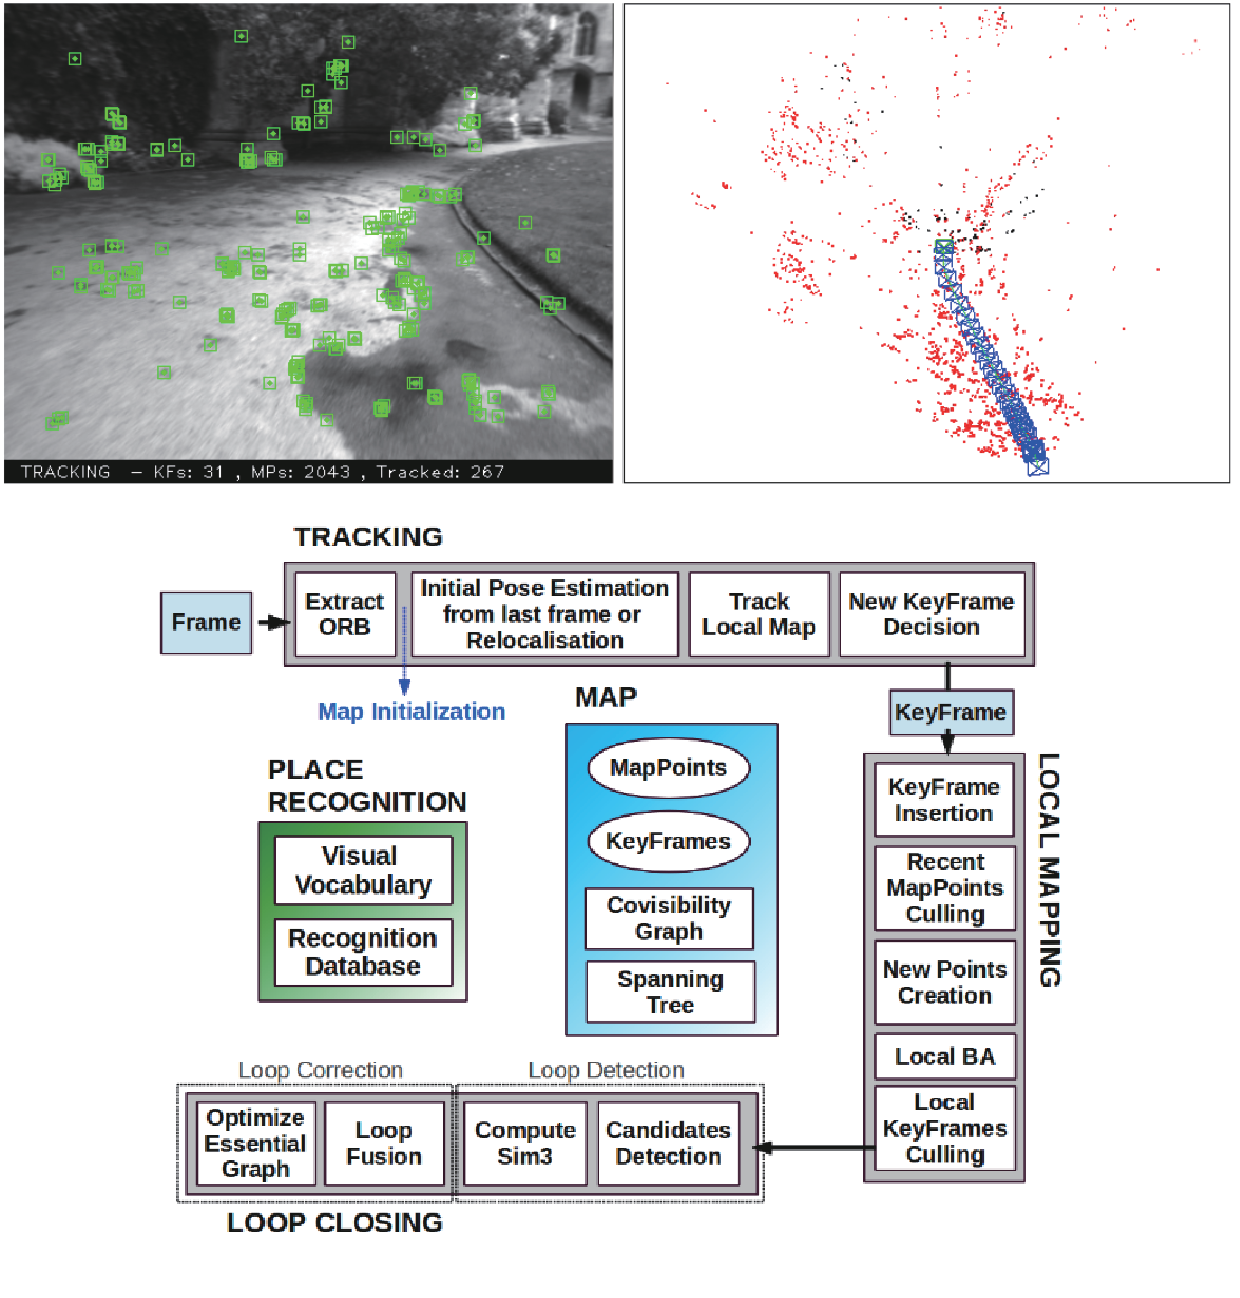
\includegraphics[width=1.0\textwidth]{past-and-future/orb-slam}
	\caption{ORB-SLAM运行截图。左侧为图像与追踪到的特征点,右侧为相机轨迹与建模的特征点地图。下方为其标志性的三线程结构。}
	\label{fig:orb-slam}
\end{figure}

\begin{enumerate}
	\item 支持单目、双目、RGB-D三种模式。这使得无论我们拿到了哪种常见的传感器,都可以先放到ORB-SLAM上测试一下,它具有良好的泛用性。
	\item 整个系统围绕ORB特征进行计算,包括视觉里程计与回环检测的ORB字典。它体现出ORB特征是现阶段计算平台的一种优秀的效率与精度之间的折中方式。ORB不像SIFT或SURF那样费时,在CPU上面即可实时计算;相比Harris角点等简单角点特征,又具有良好的旋转和缩放不变性。并且,ORB提供描述子,使我们在大范围运动时能够进行回环检测和重定位。
	\item  ORB的回环检测是它的亮点。优秀的回环检测算法保证了ORB-SLAM有效地防止累积误差,并且在丢失之后还能迅速找回,这一点许多现有的SLAM系统都不够完善。为此,ORB-SLAM在运行之前必须加载一个很大的ORB字典\mbox{文件}\footnote{目前开源版ORB-SLAM使用了文本格式的字典,改成二进制格式字典之后可以加速不少。}。
	\item ORB-SLAM创新式地使用了三个线程完成SLAM:实时跟踪特征点的Tracking线程,局部Bundle Adjustment的优化线程(Co-visibility Graph,俗称\textbf{小图}),以及全局Pose Graph的回环检测与优化线程(Essential Graph俗称\textbf{大图})。其中,Tracking线程负责对每幅新来的图像提取ORB特征点,并与最近的关键帧进行比较,计算特征点的位置并粗略估计相机位姿。小图线程求解一个Bundle Adjustment问题,它包括局部空间内的特征点与相机位姿。这个线程负责求解更精细的相机位姿与特征点空间位置。不过,仅有前两个线程,只完成了一个比较好的视觉里程计。第三个线程,也就是大图线程,对全局的地图与关键帧进行回环检测,消除累积误差。由于全局地图中的地图点太多,所以这个线程的优化不包括地图点,而只有相机位姿组成的位姿图。
	
	\hspace{2em}继PTAM的双线程结构之后,ORB-SLAM的三线程结构取得了非常好的跟踪和建图效果,能够保证轨迹与地图的全局一致性。这种三线程结构也将被后续的研究者认同和采用。
	\item ORB-SLAM围绕特征点进行了不少的优化。例如,在OpenCV的特征提取基础上保证了特征点的均匀分布,在优化位姿时使用了一种循环优化4遍以得到更多正确匹配的方法,比PTAM更为宽松的关键帧选取策略,等等。这些细小的改进使得ORB-SLAM具有远超其他方案的稳健性:即使对于较差的场景,较差的标定内参,ORB-SLAM都能够顺利地工作。
\end{enumerate}

上述这些优势使得ORB-SLAM在特征点SLAM中达到顶峰,许多研究工作都以ORB-SLAM作为标准,或者在它的基础上进行后续的开发。它的代码以清晰易读著称,有着完善的注释,可供后来的研究者进一步理解。

当然,ORB-SLAM也存在一些不足之处。首先,由于整个SLAM系统都采用特征点进行计算,我们必须对每幅图像都计算一遍ORB特征,这是非常耗时的。ORB-SLAM的三线程结构也给CPU带来了较重的负担,使得它只有在当前PC架构的CPU上才能实时运算,移植到嵌入式设备上则有一定困难。其次,ORB-SLAM的建图为稀疏特征点,目前还没有开放存储和读取地图后重新定位的功能(虽然从实现上来讲并不困难)。根据我们在建图部分的分析,稀疏特征点地图只能满足我们对定位的需求,而无法提供导航、避障、交互等诸多功能。然而,如果我们仅用ORB-SLAM处理定位问题,似乎又显得有些过于重量级了。相比之下,另外一些方案提供了更为轻量级的定位,使我们能够在低端的处理器上运行SLAM,或者让CPU有余力处理其他的事务。

\subsection{LSD-SLAM}

LSD-SLAM(Large Scale Direct monocular SLAM)是J. Engel等人于2014年提出的SLAM工作\textsuperscript{\cite{Engel2013, Engel2014}}。类比于ORB-SLAM之于特征点,LSD-SLAM则标志着单目直接法在SLAM中的成功应用。LSD-SLAM的核心贡献是将直接法应用到了半稠密的单目SLAM中。它不仅不需要计算特征点,还能构建半稠密的地图——这里半稠密的意思主要是指估计梯度明显的像素位置。它的主要优点如下:

\begin{enumerate}
	\item LSD-SLAM的直接法是针对像素进行的。作者有创见地提出了像素梯度与直接法的关系,以及像素梯度与极线方向在稠密重建中的角度关系。这些在本书的第8讲和第13讲均有讨论。不过,LSD-SLAM是在单目图像进行半稠密的跟踪,实现原理要比本书的例程更加复杂。
	\item LSD-SLAM在CPU上实现了半稠密场景的重建,这在之前的方案中是很少见到的。基于特征点的方法只能是稀疏的,而进行稠密重建的方案大多要使用RGB-D传感器,或者使用GPU构建稠密地图\textsuperscript{\cite{Kerl2013}}。TUM计算机视觉组在多年对直接法研究的基础上,实现了这种CPU上的实时半稠密SLAM。
	\item 之前也说过,LSD-SLAM的半稠密追踪使用了一些精妙的手段来保证追踪的实时性与稳定性。例如,LSD-SLAM既不是利用单个像素,也不是利用图像块,而是在极线上等距离取5个点,度量其SSD;在深度估计时,LSD-SLAM首先用随机数初始化深度,在估计完后又把深度均值归一化,以调整尺度;在度量深度不确定性时,不仅考虑三角化的几何关系,而且考虑了极线与深度的夹角,归纳成一个光度不确定性项;关键帧之间的约束使用了相似变换群及与之对应的李代数$\bm{\zeta} \in \mathfrak{sim}(3)$显式地表达出尺度,在后端优化中可以将不同尺度的场景考虑进来,减小了尺度飘移现象。
\end{enumerate}

\autoref{fig:lsd-slam}~显示了LSD的运行情况。我们可以观察一下这种微妙的半稠密地图是怎样一种介于稀疏地图与稠密地图之间的形式。半稠密地图建模了灰度图中有明显梯度的部分,显示在地图中,很大一部分都是物体的边缘或表面上带纹理的部分。LSD-SLAM对它们进行跟踪并建立关键帧,最后优化得到这样的地图。看起来比稀疏的地图具有更多的信息,但又不像稠密地图那样拥有完整的表面(稠密地图一般认为无法仅用CPU实现实时性)。

\begin{figure}[!ht]
	\centering
	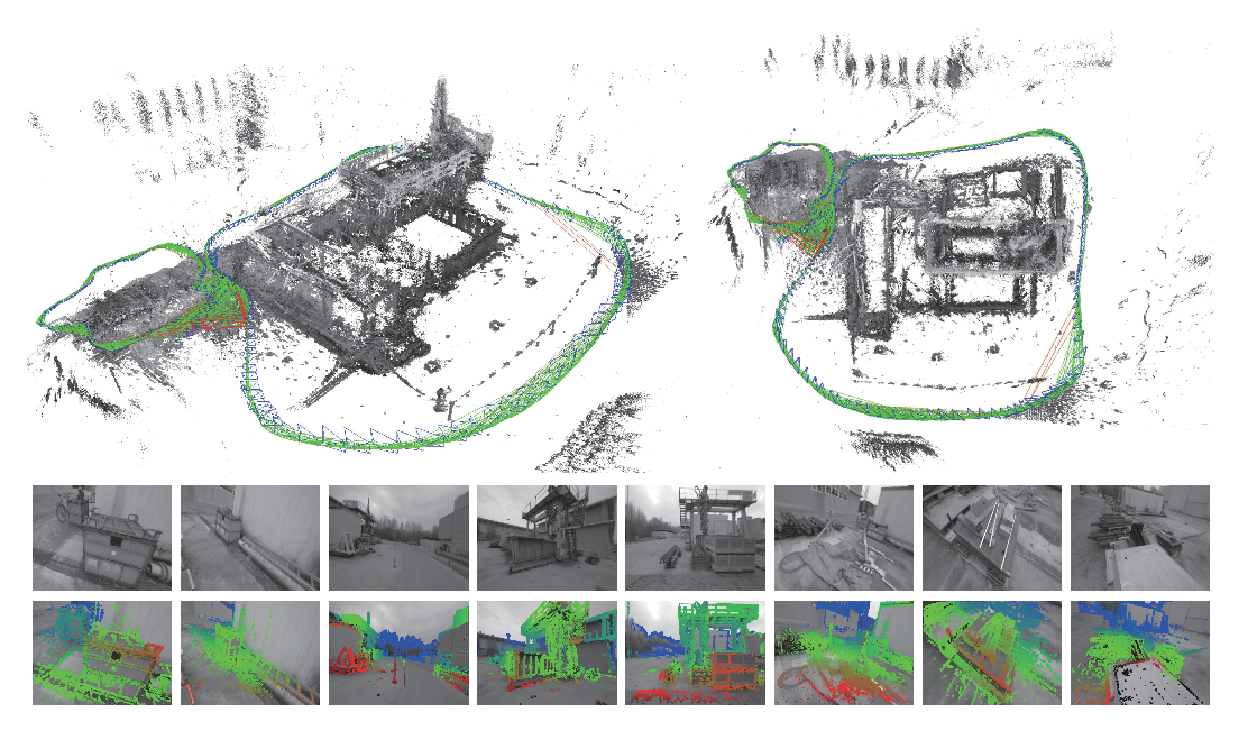
\includegraphics[width=1.0\textwidth]{past-and-future/lsd-slam}
	\caption{LSD-SLAM运行图片。上半部分为估计的轨迹与地图,下半部分为图像中被建模的部分,即具有较好的像素梯度的部分。}
	\label{fig:lsd-slam}
\end{figure}

由于LSD-SLAM使用了直接法进行跟踪,所以它既有直接法的优点(对特征缺失区域不敏感),也继承了直接法的缺点。例如,LSD-SLAM对相机内参和曝光非常敏感,并且在相机快速运动时容易丢失。另外,在回环检测部分,由于目前并没有基于直接法实现的回环检测方式,因此LSD-SLAM必须依赖于特征点方法进行回环检测,尚未完全摆脱特征点的计算。

\subsection{SVO}

SVO是Semi-direct Visual Odoemtry的缩写\textsuperscript{\cite{Forster2014}}。它是由Forster等人于2014年提出的一种基于稀疏直接法的视觉里程计。按作者的称呼应该叫“半直接”法,然而按照本书的理念框架,称为“稀疏直接法”可能更好一些。\textbf{半直接}在原文中的意思是指特征点与直接法的混合使用:SVO跟踪了一些关键点(角点,没有描述子),然后像直接法那样,根据这些关键点周围的信息估计相机运动及其位置(如\autoref{fig:lsd-slam}所示)。在实现中,SVO使用了关键点周围的$4\times4$的小块进行块匹配,估计相机自身的运动。

相比于其他方案,SVO的最大优势是速度极快。由于使用稀疏的直接法,它既不必费力去计算描述子,也不必处理像稠密和半稠密那么多的信息,因此,即使在低端计算平台上也能达到实时性,而在PC平台上则可以达到每秒100多帧的速度。在后续的SVO 2.0中,速度更达到了惊人的每秒400帧。这使得SVO非常适用于计算平台受限的场合,例如无人机、手持AR/VR设备的定位。无人机也是作者开发SVO的目标应用平台。

\begin{figure}[H]
	\centering
	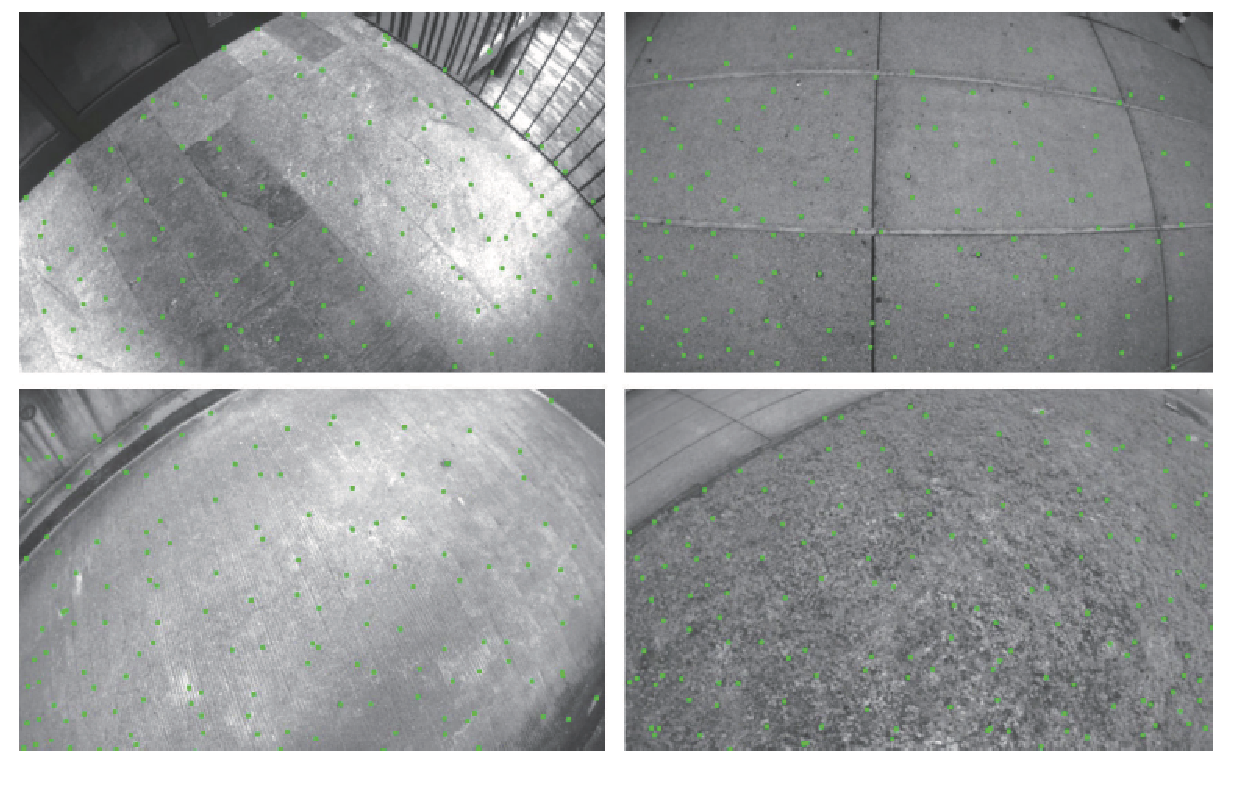
\includegraphics[width=1.0\textwidth]{past-and-future/svo}
	\caption{SVO跟踪关键点的图片。}
	\label{fig:svo}
\end{figure}

SVO的另一创新之处是提出了深度滤波器的概念,并推导了基于均匀−高斯混合分布的深度滤波器。这在本书的第13讲有提及,但由于原理较为复杂,我们没有详细解释。SVO将这种滤波器用于关键点的位置估计,并使用了逆深度作为参数化形式,使之能够更好地计算特征点位置。

开源版的SVO代码清晰易读,十分适合读者作为第一个SLAM实例进行分析。不过,开源版SVO也存在一些问题:

\begin{enumerate}
	\item 由于目标应用平台为无人机的俯视相机,其视野内的物体主要是地面,而且相机的运动主要为水平和上下的移动,SVO的许多细节是围绕这个应用设计的,这使得它在平视相机中表现不佳。例如,SVO在单目初始化时,使用了分解$\bm{H}$矩阵而不是传统的$\bm{F}$或$\bm{E}$矩阵的方式,这需要假设特征点位于平面上。该假设对俯视相机是成立的,但对平视相机通常是不成立的,可能导致初始化失败。再如,SVO在关键帧选择时,使用了平移量作为确定新的关键帧的策略,而没有考虑旋转量。这同样在无人机俯视配置下是有效的,但在平视相机中则会容易丢失。所以,如果读者想要在平视相机中使用SVO,必须自己加以修改。
	\item SVO为了速度和轻量化,舍弃了后端优化和回环检测部分,也基本没有建图功能。这意味着SVO的位姿估计必然存在累积误差,而且丢失后不太容易进行重定位(因为没有描述子用来回环检测)。所以,我们称它为一个VO,而不是称它为完整的SLAM。
\end{enumerate}

\subsection{RTAB-MAP}

介绍了几款单目SLAM方案后,我们再来看一些RGB-D传感器上的SLAM方案。相比于单目和双目,RGB-D SLAM的原理要简单很多(尽管实现上不一定),而且能够在CPU上实时建立稠密的地图。

RTAB-MAP(Real Time Appearance-Based Mapping)\textsuperscript{\cite{Labbe2014}}是RGB-D SLAM中比较经典的一个方案。它实现了RGB-D SLAM中所有应该有的东西:基于特征的视觉里程计、基于词袋的回环检测、后端的位姿图优化,以及点云和三角网格地图。因此,RTAB-MAP给出了一套完整的(但有些庞大的)RGB-D SLAM方案。目前我们已经可以直接从ROS中获得其二进制程序,此外,在Google Project Tango上也可以获取其App使用(如\autoref{fig:rtabmap}~所示)。

\begin{figure}[!ht]
	\centering
	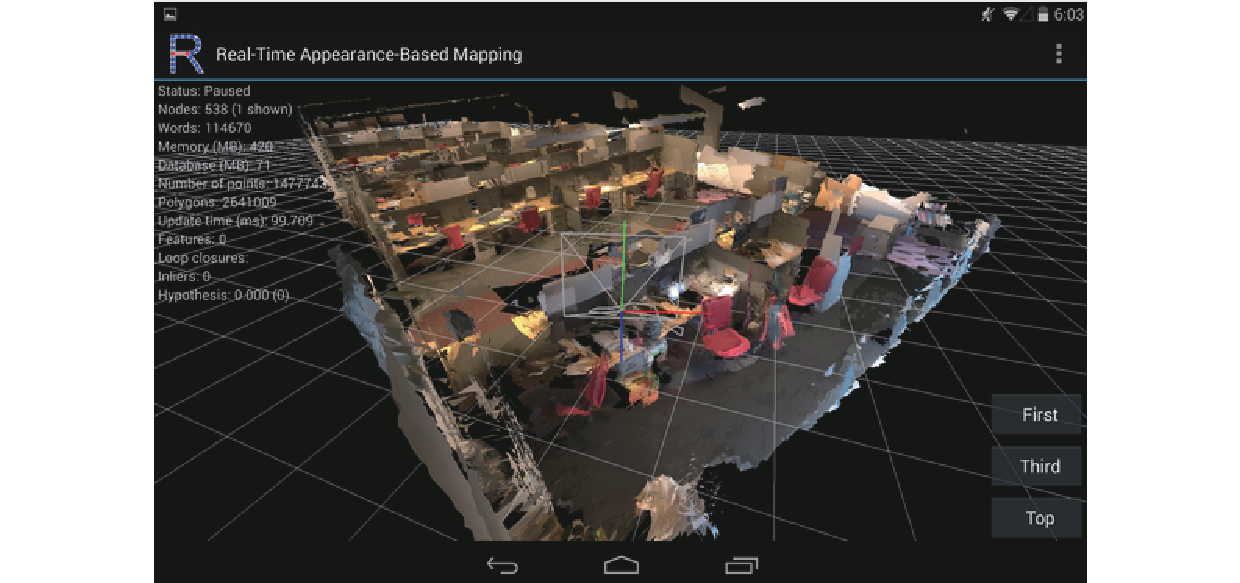
\includegraphics[width=1.0\textwidth]{past-and-future/rtabmap}
	\caption{RTAB-MAP在Google Project Tango上的运行样例。}
	\label{fig:rtabmap}
\end{figure}

RTAB-MAP支持一些常见的RGB-D和双目传感器,像Kinect、Xtion等,且提供实时的定位和建图功能。不过由于集成度较高,使得其他开发者在它的基础上进行二次开发变得困难,所以RTAB-MAP更适合作为SLAM应用而非研究使用。

\subsection{其他}
除了这些开源方案之外,读者还能在\url{openslam.org}之类的网站上找到许多其他的研究,例如,DVO-SLAM\textsuperscript{\cite{Kerl2013a}}、RGBD-SLAM-V2\textsuperscript{\cite{Endres2014}}、DSO\textsuperscript{\cite{Engel2016}},以及一些Kinect Fusion相关的工作,等等。随着时代发展,更新颖、更优秀的开源SLAM作品亦将出现在人们的视野中,限于篇幅这里就不逐一介绍了。
	
%\subsection{OKVis}
%在视觉SLAM之外,还有一个称为VIO
%\subsection{未开源的一些工作}

\section{未来的SLAM话题}
看过了现有的方案,我们再来讨论一些未来的发展方向\footnote{这里有一部分是笔者个人的理解,不一定完全正确。}。大体上讲,SLAM将来的发展趋势有两大类:一是朝轻量级、小型化方向发展,让SLAM能够在嵌入式或手机等小型设备上良好运行,然后考虑以它为底层功能的应用。毕竟,大部分场合中,我们的真正目的都是实现机器人、AR/VR设备的功能,比如说运动、导航、教学、娱乐,而SLAM是为上层应用提供自身的一个位姿估计。在这些应用中,我们不希望SLAM占用所有计算资源,所以对SLAM的小型化和轻量化有非常强烈的需求。另一方面则是利用高性能计算设备,实现精密的三维重建、场景理解等功能。在这些应用中,我们的目的是完美地重建场景,而对于计算资源和设备的便携性则没有多大限制。由于可以利用GPU,这个方向和深度学习亦有结合点。

\subsection{视觉+惯性导航SLAM}

首先,我们要谈一个有很强应用背景的方向:视觉−惯性导航融合SLAM方案。实际的机器人也好,硬件设备也好,通常都不会只携带一种传感器,往往是多种传感器的融合。学术界的研究人员喜爱“大而且干净的问题”(Big Clean Problem),比如说仅用单个摄像头实现视觉SLAM。但产业界的朋友们则更注重让算法更加实用,不得不面对一些复杂而琐碎的场景。在这种应用背景下,用视觉与惯性导航融合进行SLAM成为了一个关注热点。

惯性传感器(IMU)能够测量传感器本体的角速度和加速度,被认为与相机传感器具有明显的互补性,而且十分有潜力在融合之后得到更完善的SLAM系统\textsuperscript{\cite{Gui2015}}。为什么这么说呢?

\begin{enumerate}
	\item IMU虽然可以测得角速度和加速度,但这些量都存在明显的漂移(Drift),使得积分两次得到的位姿数据非常不可靠。好比说,我们将IMU放在桌上不动,用它的读数积分得到的位姿也会漂出十万八千里。但是,对于短时间内的快速运动,IMU能够提供一些较好的估计。这正是相机的弱点。
	
	\clearpage
	\hspace{2em}当运动过快时,(卷帘快门的)相机会出现运动模糊,或者两帧之间重叠区域太少以至于无法进行特征匹配,所以纯视觉SLAM非常害怕快速的运动。而有了IMU,即使在相机数据无效的那段时间内,我们也能保持一个较好的位姿估计,这是纯视觉SLAM无法做到的。
	
	\item 相比于IMU,相机数据基本不会有漂移。如果相机放在原地固定不动,那么(在静态场景下)视觉SLAM的位姿估计也是固定不动的。所以,相机数据可以有效地估计并修正IMU读数中的漂移,使得在慢速运动后的位姿估计依然有效。
	
	\item 当图像发生变化时,本质上我们没法知道是相机自身发生了运动,还是外界条件发生了变化,所以纯视觉SLAM难以处理动态的障碍物。而IMU能够感受到自己的运动信息,从某种程度上减轻动态物体的影响。
\end{enumerate}

总而言之,我们看到IMU为快速运动提供了较好的解决方式,而相机又能在慢速运动下解决IMU的漂移问题——在这个意义下,它们二者是互补的。

\begin{figure}[!thp]
	\centering
	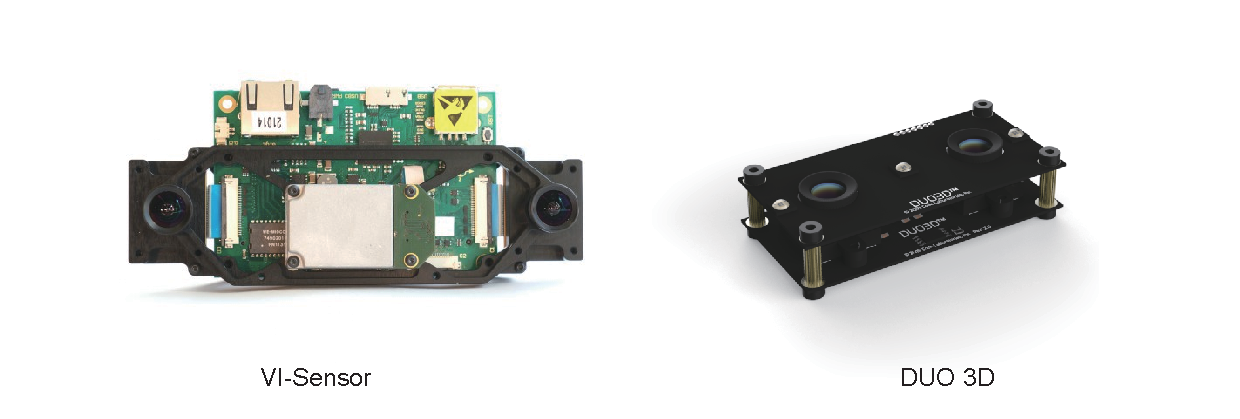
\includegraphics[width=1.0\textwidth]{past-and-future/visensor}
	\caption{越来越多的相机开始集成IMU设备。}
	\label{fig:visensor}
\end{figure}

当然,虽然说得很好听,不管是理论还是实践,VIO(Visual Inertial Odometry)都是相当复杂的。其复杂性主要来源于IMU测量加速度和角速度这两个量的事实,所以不得不引入运动学计算。目前VIO的框架已经定型为两大类:松耦合(Loosely Coupled)和紧耦合(Tightly Coupled)\textsuperscript{\cite{Martinelli2014}}。松耦合是指IMU和相机分别进行自身的运动估计,然后对其位姿估计结果进行融合。紧耦合是指把IMU的状态与相机的状态合并在一起,共同构建运动方程和观测方程,然后进行状态估计——这和我们之前介绍的理论非常相似。我们可以预见,紧耦合理论也必将分为基于滤波和基于优化两个方向。在滤波方面,传统的EKF\textsuperscript{\cite{Bloesch2015}}以及改进的MSCKF(Multi-State Constraint KF)\textsuperscript{\cite{Li2013}}都取得了一定的成果,研究者对EKF也进行了深入的讨论(例如能观性\textsuperscript{\cite{Huang2014}});优化方面亦有相应的方案\textsuperscript{\cite{Leutenegger2015, Forster2015}}。值得一提的是,尽管在纯视觉SLAM中优化方法已经占了主流,但在VIO中,由于IMU的数据频率非常高,对状态进行优化需要的计算量就更大,因此目前仍处于滤波与优化并存的阶段\textsuperscript{\cite{Tkocz2015, Usenko2016}}。由于过于复杂,限于篇幅,这里就只能大概地介绍一下这个方向了。

VIO为将来SLAM的小型化与低成本化提供了一个非常有效的方向。而且结合稀疏直接法,我们有望在低端硬件上取得良好的SLAM或VO效果,是非常有前景的。

\subsection{语义SLAM}
SLAM的另一个大方向就是和深度学习技术结合。到目前为止,SLAM的方案都处于特征点或者像素的层级。关于这些特征点或像素到底来自于什么东西,我们一无所知。这使得计算机视觉中的SLAM与我们人类的做法不怎么相似,至少我们自己从来看不到特征点,也不会去根据特征点判断自身的运动方向。我们看到的是一个个物体,通过左右眼判断它们的远近,然后基于它们在图像当中的运动推测相机的移动。

很久之前,研究者就试图将物体信息结合到SLAM中。例如文献\cite{Nuechter2008, Civera2011, Koppula2011, Anand2012}中就曾把物体识别与视觉SLAM结合起来,构建带物体标签的地图。另一方面,把标签信息引入到BA或优化端的目标函数和约束中,我们可以结合特征点的位置与标签信息进行优化\textsuperscript{\cite{Fioraio2013}}。这些工作都可以称为语义SLAM。综合来说,SLAM和语义的结合点主要有两个方面\textsuperscript{\cite{Cadena2016}}:

\begin{enumerate}
	\item 语义帮助SLAM。传统的物体识别、分割算法往往只考虑一幅图,而在SLAM中我们拥有一台移动的相机。如果我们把运动过程中的图片都带上物体标签,就能得到一个带有标签的地图。另外,物体信息亦可为回环检测、BA优化带来更多的条件。 
	\item SLAM帮助语义。物体识别和分割都需要大量的训练数据。要让分类器识别各个角度的物体,需要从不同视角采集该物体的数据,然后进行人工标定,非常辛苦。而SLAM中,由于我们可以估计相机的运动,可以自动地计算物体在图像中的位置,节省人工标定的成本。如果有自动生成的带高质量标注的样本数据,能够很大程度上加速分类器的训练过程。
\end{enumerate}

\begin{figure}[!thp]
	\centering
	\includegraphics[width=1.0\textwidth]{past-and-future/semantic-slam}
	\caption{语义SLAM的一些结果,左图和右图分别来自文献\cite{Anand2012, Salas-Moreno2014}。}
	\label{fig:semantic-slam}
\end{figure}

在深度学习广泛应用之前,我们只能利用支持向量机、条件随机场等传统工具对物体或场景进行分割和识别,或者直接将观测数据与数据库中的样本进行比较\textsuperscript{\cite{Salas-Moreno2013, Salas-Moreno2014}},尝试构建语义地图\textsuperscript{\cite{Anand2012, Stueckler2012, Kostavelis2013, Couprie2013}}。由于这些工具本身在分类正确率上存在限制,所以效果也往往不尽如人意。随着深度学习的发展,我们开始使用网络,越来越准确地对图像进行识别、检测和分割\textsuperscript{\cite{Deng2009, Krizhevsky2012, He2015, Ren2015, Long2014, Zheng2015}}。这为构建准确的语义地图打下了更好的基础\textsuperscript{\cite{Gupta2014}}。我们正看到,逐渐开始有学者将神经网络方法引入到SLAM中的物体识别和分割,甚至SLAM本身的位姿估计与回环检测中\textsuperscript{\cite{Konda2015, Kendall2015, Hou2015}}。虽然这些方法目前还没有成为主流,但将SLAM与深度学习结合来处理图像,亦是一个很有前景的研究方向。

\subsection{SLAM的未来}
除此之外,基于线/面特征的SLAM\textsuperscript{\cite{An2012, Zhou2015, Benedettelli2012}}、动态场景下的SLAM\textsuperscript{\cite{Saarinen2013, Maddern2012,  Wang2008}}、多机器人的SLAM\textsuperscript{\cite{Zou2013, Gil2010a, Vidal-Calleja2011}},等等,都是研究者感兴趣并发力的地方。按照文献\cite{Cadena2016}的观点,视觉SLAM经过了三个大时代:提出问题、寻找算法、完善算法。而我们目前正处于第三个时代,面对着如何在已有的框架中进一步改善,使视觉SLAM系统能够在各种干扰的条件下稳定运行。这一步需要许多研究者的不懈努力。

当然,没有人能够预测未来,我们也说不准会不会突然有一天,整个框架都被新的技术推倒重写。不过即使是那样,今天我们的付出仍将是有意义的。没有今天的研究,也就不会有将来的发展。最后,希望读者能在读完本书之后,对现有的整个SLAM系统有了充分的认识。我们也期待你能够为SLAM研究做出贡献!

\section*{习题}
\begin{enumerate}
	\item 选择本讲提到的任意一个开源SLAM系统,在你的机器上编译运行它,直观体验其过程。
	\item 你应该已经能够看懂绝大多数SLAM相关论文了。拿起纸和笔,开始你的研究吧!
\end{enumerate}
